\documentclass[10pt,twocolumn,letterpaper]{article}

\usepackage{cvpr}
\usepackage{times}
\usepackage{epsfig}
\usepackage{graphicx}
\usepackage{amsmath}
\usepackage{amssymb}
\usepackage{mathrsfs}
\usepackage{mathtools}
\usepackage{subfigure}
\DeclareMathOperator*{\argmin}{arg\,min}
% Include other packages here, before hyperref.

% If you comment hyperref and then uncomment it, you should delete
% egpaper.aux before re-running latex.  (Or just hit 'q' on the first latex
% run, let it finish, and you should be clear).
\usepackage[pagebackref=true,breaklinks=true,letterpaper=true,colorlinks,bookmarks=false]{hyperref}

\newcommand{\deva}[1]{\textcolor{red}{[Deva: #1]}}


% \cvprfinalcopy % *** Uncomment this line for the final submission

\def\cvprPaperID{****} % *** Enter the CVPR Paper ID here
\def\httilde{\mbox{\tt\raisebox{-.5ex}{\symbol{126}}}}

% Pages are numbered in submission mode, and unnumbered in camera-ready
\ifcvprfinal\pagestyle{empty}\fi
\begin{document}

%%%%%%%%% TITLE
\title{DAG-CNNs for multi-scale recognition}

\author{First Author\\
Institution1\\
Institution1 address\\
{\tt\small firstauthor@i1.org}
% For a paper whose authors are all at the same institution,
% omit the following lines up until the closing ``}''.
% Additional authors and addresses can be added with ``\and'',
% just like the second author.
% To save space, use either the email address or home page, not both
\and
Second Author\\
Institution2\\
First line of institution2 address\\
{\tt\small secondauthor@i2.org}
}

\maketitle
%\thispagestyle{empty}

%%%%%%%%% ABSTRACT
\begin{abstract}
While Deep Convolutional Neural Network (CNN) encodes multi-scale features with their spatial locations, Bag-of-feature representations are more invariant to spatial translations. In this paper, we propose a CNN architecture transformation schema that extracts multi-scale CNN representations with spatial invariance. By directly chaining multiple average-pooled rectified linear units (ReLU) to the final layer of scoring function, we explicitly learn an augmented model from multi-scale activations. We term this transformation Bag-of-Multi-Sale-Activation (BoMSA) Augmentation. The BoMSA augmented model can be trained from scratch or built upon existing pre-trained models, which makes the augmentation more flexible. BoMSA augmentation is also model-independent and can be easily adapted to existing models. Experimental results show consistent improvements achieved by incorporating the BoMSA representation on various models in the literature.  

\end{abstract}

%%%%%%%%% BODY TEXT
\section{Introduction}


\begin{figure}[t!]
\centering
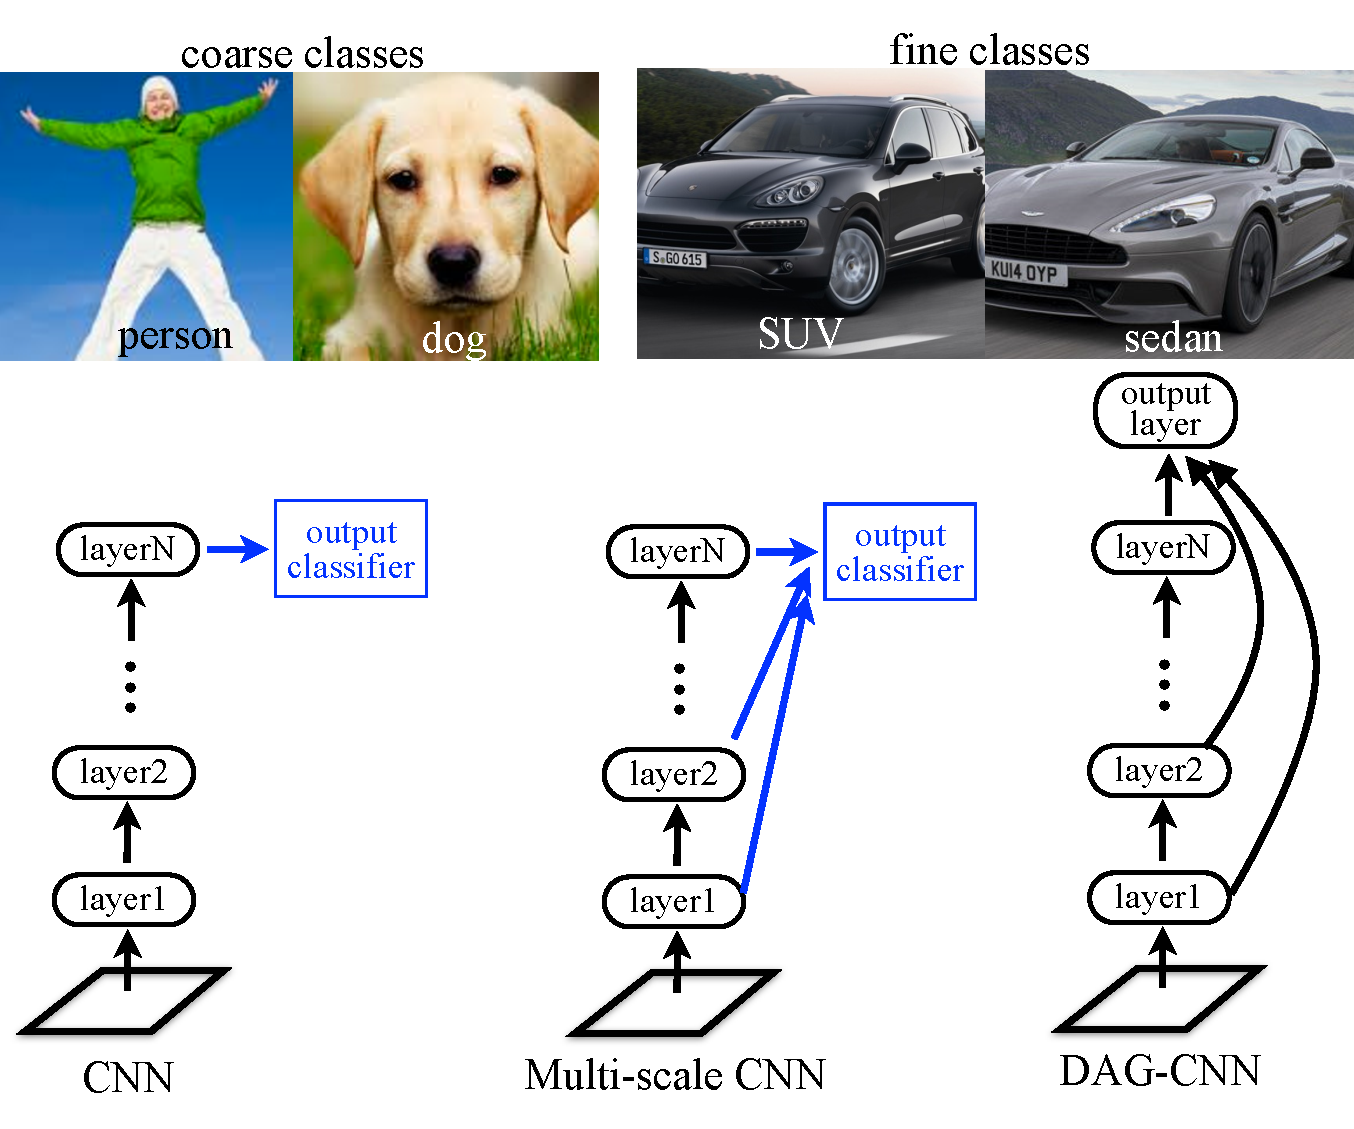
\includegraphics[width=\columnwidth]{fig/deva_splash}
\caption{Recognition typically require features at multiple scales. Distinguishing a person versus dog requires highly invariant features robust to the deformation of each category. On the other hand, fine-grained recognition likely requires detailed shape cues to distinguish models of cars ({\bf top}). We use these observations to revisit deep convolutional neural net (CNN) architectures. Typical approaches train a classifier using features from a single output layer ({\bf left}). We extract multi-scale features from multiple layers to simultaneously distinguish coarse and fine classes. Such features come ``for free'' since they are already computed during the feed-forward pass ({\bf middle}). Interestingly, the entire multi-scale predictor is still a feed-forward architecture that is no longer chain-structured, but a directed-acyclic graph (DAG) ({\bf right}). We show that DAG-CNNs can be discriminatively trained in an end-to-end fashion, yielding state-of-the-art recognition results across various recognition benchmarks.  DAG-CNNs address some well-known challenges with CNNs such as ``vanishing gradients''~\cite{bengio1994learning}. Lower layers in a DAG-CNN still receive a strong gradient signal during learning because they are directly tied to the output layer, making them easier to train.
\label{fig:splash}}
\end{figure}

Deep convolutional neural nets (CNNs), pioneered by Lecun and collaborators~\cite{lecun1998gradient}, now produce state-of-the-art performance on many visual recognition tasks~\cite{AlexNet, overfeat, veryDeep, GoogLeNet, nin}. An attractive property is that appear to serve as universal feature extractors, either as ``off-the-shelf'' features or through a small amount of ``fine tuning''. CNNs trained on particular tasks such as large-scale image classification~\cite{ImageNet} {\em transfer} extraordinarily well to other tasks such as object detection~\cite{rcnn}, scene recognition~\cite{zhoulearning}, image retrieval~\cite{Gong14}, etc \cite{cnn_baseline}.

{\bf Hierarhical  models:}  CNNs are 
hierarchical feed-forward architectures that compute progressively invariant representations of the input image. However, the appropriate level of invariance might be task-dependent. Distinguishing people and dogs requires a representation that is robust to large spatial deformations, since people and dogs can articulate. However, fine-grained categorization of car models (or bird species) requires fine-scale features that capture subtle shape cues. We argue that a universal architecture capable of both tasks must employ some form of multi-scale features for output prediction.

{\bf Multi-scale features:} We introduce multi-scale CNN architectures that use features at multiple scales for output prediction (Fig.~\ref{fig:splash}). From one perspective, our architectures are quite simple. Typical approaches train a output predictor (e.g., a linear SVM) using features extracted from a single output layer. Instead, one can train an output predictor using features extracted from multiple layers. Note that these features come ``for free''; they are already computed in a standard feed-forward pass. 

{\bf Marginal activations:} One difficulty with multi-scale approaches is feature dimensionality - the total number of features across all layers can easily reach hundred of thousands. This makes training even linear models difficult and prone to overfitting. Instead, we use marginal activations computed from sum (or max) pooling across all spatial locations in a given activation layer. From this perspective, our models are similar to those that compute multi-scale features with spatial pooling, including multi-scale templates~\cite{felzenszwalb2008discriminatively}, orderless models\cite{Gong14}, spatial pyramids~\cite{spatial_pyramid}, and bag-of-words~\cite{sivic2003video}.

{\bf DAG-CNN:} Our multi-scale model differs from such past work in one notable aspect. Our model is still a feed-forward CNN that is no longer chain-structured, but a directed-acyclic graph (DAG). DAG-structured CNNs can be discriminatively trained in an end-to-end fashion, allowing us to learn multiscale representations. Multi-scale learning addresses one well-known difficulty of CNNs - the ``vanishing gradient'' problem~\cite{bengio1994learning}. During gradient-based learning, the gradient signal becomes progressively diluted as one back-propogates it through multiple layers, such that the bottom-most layer receives essentially no updates. Our multi-scale DAG structure connects all activation layers directly to the output, ensuring they all receive a strong gradient signal during learning. 

%yeilding state-of-the-art recognition results across various recognition benchmarks. 

% Trained with large number of instances, (such as ImageNet~\cite{ImageNet}), CNN is also an excel candidate for off-the-shelf feature extractions, results in outstanding performance in various recognition tasks~\cite{cnn_baseline}. In the meantime, a considerable amount of effort is spent on how to further improve the performance of CNN. On one hand, many are focus on techniques to efficiently and effective train a CNN. A good initialization need to be carefully selected~\cite{diff_cnn} in the beginning. Data augmentation~\cite{AlexNet} is recommended to improve the model performance as well. Drop-out~\cite{dropout} and momentum~\cite{momentum} are also necessary to prevent over-fitting and obtain superior models. On the other hand, different model components and architectures are proposed. Rectified linear units (ReLU)~\cite{AlexNet} add non-linearity and enrich the model complexity. Different pooling method, such as Distance Transform Pooling~\cite{dist_trans}, is adopted in~\cite{dpm_is_cnn}, allowing local deformations, as in the widely-used deformable part-based model (DPM)~\cite{dpm}. \cite{veryDeep} adopts a small $3\times 3$ receptive field to deepen the model, while maintaining less parameters. A network in network~\cite{nin} is proposed to enhance model discriminability for local patches within the receptive field. The award winning GoogLeNet~\cite{GoogLeNet} uses an \textit{Inception} model that is based on the Hebbian principle~\cite{Hebb}, \ie, neurons that fire together, wire together, the theoretical proof of which is provided by~\cite{dnn_proof} under constraints. 

%One question to ponder: is there any model-independent potential that is yet to be discovered. Although allowing local deformation, CNN encodes the the spatial information of multi-scale features. Conversely, by ignoring the spatial location of features, bag-of-feature like techniques~\cite{spatial_pyramid} achieves transformation invariance to some extend. As pointed out in~\cite{Gong14}, combining both type of features results in a better representation for recognition tasks with large variations, such as Scene classification~\cite{SUN397,MIT67}. Traditionally, when CNN is used for feature extraction, the activation of the first fully-connected (FC) layer is usually considered as the feature~\cite{overfeat, Gong14}. Using an off-the-shelf deep CNN model,~\cite{Gong14} explicitly extracts image patches from three scales and computes the feed-forward CNN activations for each patch for feature extraction. This algorithm is cumbersome due to the computation of multiple patches for one image. Besides, it can only encode the multi-scale features to a certain extend limited by the burden of the post processing, \ie, K-means and Principle Component Analysis (PCA). As a matter of fact, CNN feature is meant to encode multi-scale feature at each convolutional (Conv.) layer. Therefore, there is no need to extract multi-scale patches and only one feed-forward computation is sufficient to capture the activations of multi-scale features for one input image. 

\begin{figure*}[htbp]
\centering
	\subfigure[low-level feature is preferred]{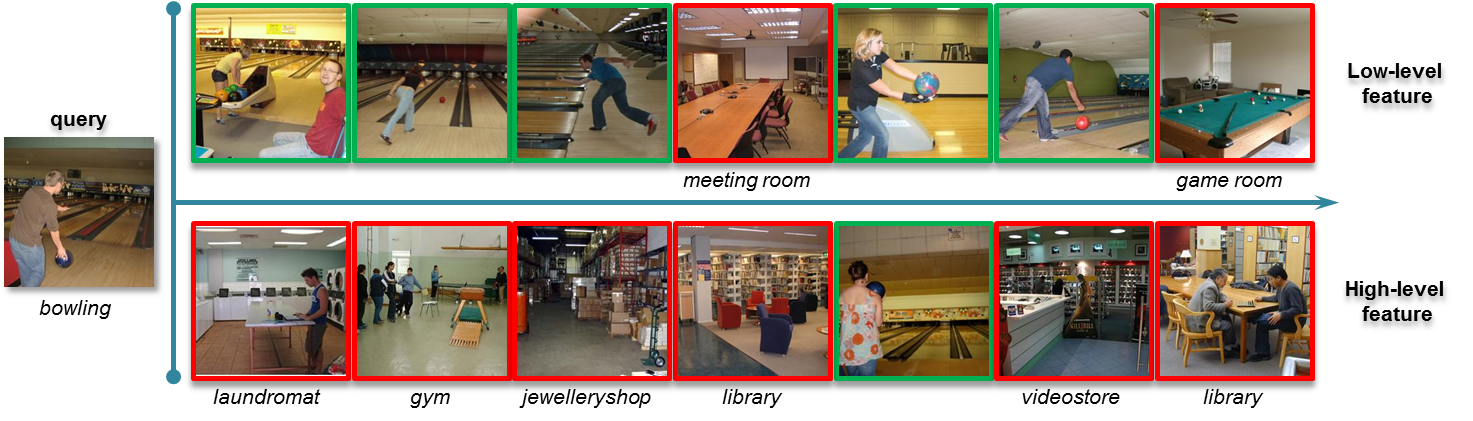
\includegraphics[width=.9\textwidth]{fig/moti_low_better.png}\label{fig:moti_low}}
	\subfigure[high-level feature is preferred]{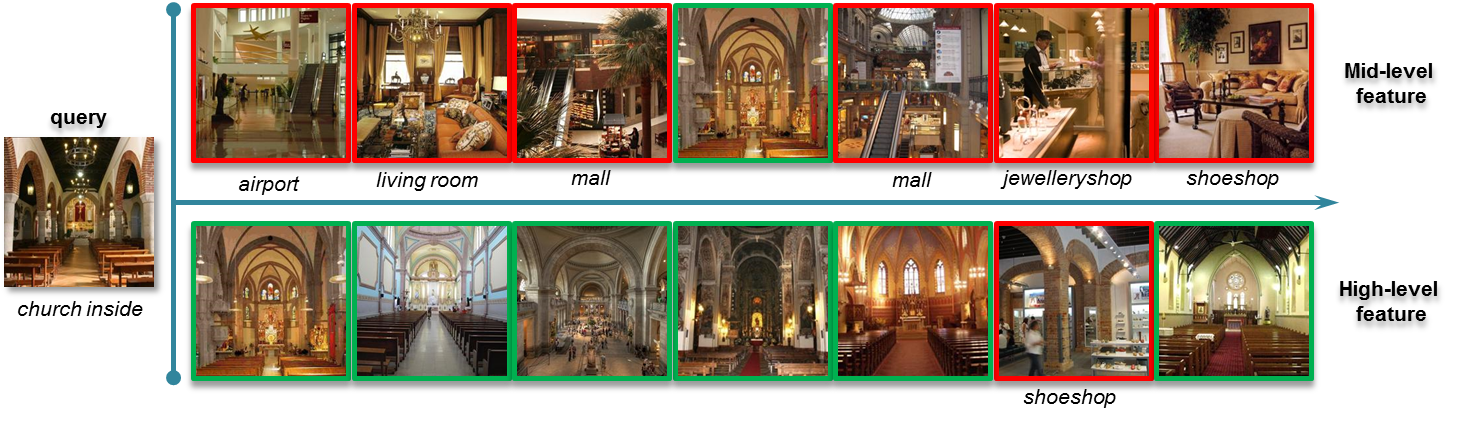
\includegraphics[width=.9\textwidth]{fig/moti_high_better.png}\label{fig:moti_high}}

\caption{Retrieval results using euclidean distance for both low- and high-level features on MIT67~\cite{MIT67}. \textit{Green} (\textit{Red}) box means correct (wrong) results. The correct label for wrong retrievals are provided. The retrieval results are displayed such that the left-most image has the closest distance to the query, and vice versa. This observation shows that both low- and high-level features are dispensable for a better representation.}

\label{fig:moti}
\end{figure*}


%In this paper, we first conducted an empirical analysis on the feature discriminativeness of every unit of CNN model. By average-pooling at each layer, the output ignores global spatial information and results in a bag-of-feature representation. The bag-of-feature from ReLU is then found to carry the most performance gain at each layer. We have also observed a synergy of multi-scale activations results in a better discriminative representation. These observations tie closely to the vanishing gradient~\cite{diff_cnn} issue in the deep CNN literature. During the training of a CNN, the top layer can be easily saturated. The gradients in the back-propagation algorithm will not effective reach the lower levels, resulting in a model that focuses more high-level features. Thus, we proposed a model augmentation schema, BoMSA, that chains the ReLU at each layer to the ultimate loss function. This augmentation approach is not confined by model variations and can be applied to existing pre-trained models or re-training the model from the ground up. By explicitly linking the lower layers to the decision layer, we gear the training towards the bag-of-activations from all layers. Thus, the augmented model is designed to be robust to spatial translations while maintaining its discriminative power in the multi-scale fashion.

{\bf DAG-structured Neural Networks:} DAG-structured neural nets have been previously explored in the context of recurrent neural nets \cite{baldi2003principled,graves2009offline}. Recurrent neural nets use feedback to capture dynamic states, and so typically cannot be processed with feedforward computations. Previous work has also shown that long-range connections between neural layers can eliminate the vanshing gradient problem, but this is done in the context of memory-based networks~\cite{hochreiter1997long}. We make use of DAG structures to efficiently encode multi-scale features in a simpler feed-forward network.

{\bf Overview:} We motivate our multi-scale DAG-CNN model in \ref{sec:approach}, describe the full architecture in Sec.~\ref{sec:ana}, and conclude with numerous benchmark results in Sec.~\ref{sec:exp}. We evaluate multi-scale DAG-structured variants of existing CNN architectures (\eg, Caffe~\cite{Caffe}, Deep19~\cite{veryDeep}) on a variety of scene recognition benchmarks including SUN397~\cite{SUN397}, MIT67~\cite{MIT67}, Scene15~\cite{Scene15}. We observe a consistent improvement regardless of the underlying CNN architecture, producing state-of-the-art results on all 3 datasets.

%A consistent performance improvement is observed of our multi-scale representation over the best discriminative single-scale feature. 
%The rest of the paper is organized as follows: we motivate and describe our model augmentation approach in Sec.~
%\ref{sec:approach}. An in-depth analysis is provided in Sec.~\ref{sec:ana}. Systematic experimental results are included in Sec.~\ref{sec:exp}. 


%-------------------------------------------------------------------------
%-------------------------------------------------------------------------
\section{Motivation\label{sec:approach}}
In this section, we motivate our multiscale architecture with a simple empirical analysis of existing CNN architectures, 
%We seek to discover a model-independent augmentation approach that enable the model with multi-scale feature representation. We first provide our motivation based on empirical studies on the discrimintiveness of individual feature at various scales as well as multi-scale features. We then describe our model augmentation technique. 
%In this work, we consider two models in the literature, 
namely Caffe and Deep19. Caffe~\cite{Caffe} is a broadly used CNN toolbox. It includes a pre-trained model ``AlexNet''~\cite{AlexNet} model, learned with millions of images from the ImageNet dataset~\cite{ImageNet}. This model has 6 conv. layers and 2 fully-connected (FC) layers. Deep19~\cite{veryDeep} uses very small $3\times 3$ receptive fields, but an increased number of layers -- 19 layers (16 conv. and 3 FC layers). This model produced state-of-the-art performance in ILSVRC-2014 classification challenge~\cite{ILSVRC14}. 
We evaluate both models on the heavily benchmarked MIT Indoor Scene (MIT67) dataset~\cite{MIT67}.

%We intend to demonstrate the consistency and model-independence of our observations and approach. We have conducted experiments on several CNN models and observed similar patterns. Due to limited space, we only provide the analysis of the aforementioned Caffe and Deep19 models as exemplars in the rest of the paper. 

%-------------------------------------------------------------------------
%\subsection{Single-scale classificationScale\label{sec:indi_scale}}

{\bf Single-scale classification:} Following past work \cite{cnn_baseline}, we train a linear SVM classifier using features extracted from a particular layer. We specifically train $K=67$ 1-vs-all linear classifiers.
We plot the performance of single-layer classifiers in Fig.~\ref{fig:layer_MIT67}. The detailed parameter options for both Caffe and Deep19 models are described later in Sec.~\ref{sec:exp}. As past work has pointed out, we see a general increase in performance as we use higher-level (more invariant) features. We do see a slight improvement at each nonlinear activation (RelU) layer. This makes sense as this layer introduces a nonlinear rectification operation $\max(0,x)$, while other layers (such an convolutional or sum-pooling) are linear operations that can be learned by a linear predictor.
%As seen in Fig.~\ref{fig:layer_MIT67}, in general, the discriminativeness of the model increases as the layer becomes higher. More importantly, we observe significant improvement resulting from each Rectified Linear Units (ReLU). As described in~\cite{ReLU,AlexNet}, ReLU models a neuron's output $r$ as a mapping of its input $x$ with the non-saturating nonlinearity $r(x)=\max (0,x)$. We are then motivated to choose the output of the ReLU layer due to this nonlinearity it introduces to the CNN architecture, which boosts the discriminative power of the model. 

\begin{figure}[htbp]
\centering
	\subfigure[Caffe]{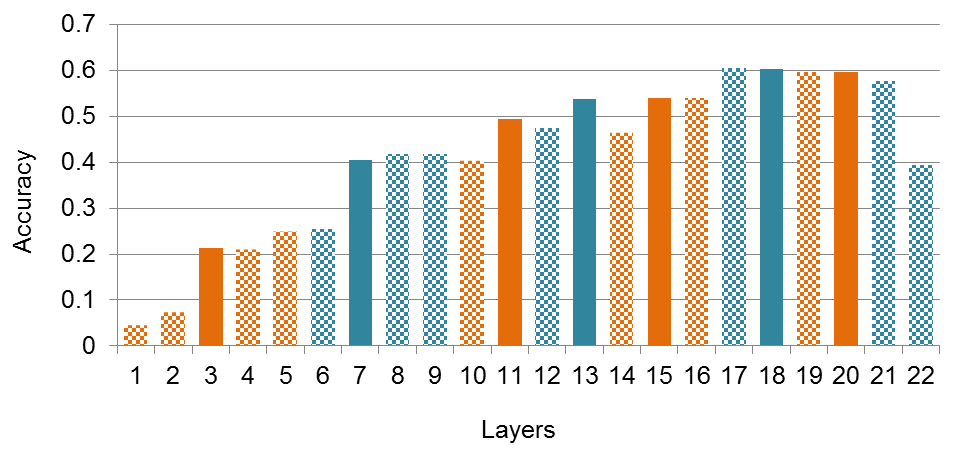
\includegraphics[width=\columnwidth]{fig/fig_layer_caffe.png}\label{fig:layer_caffe}}
	\subfigure[Deep19]{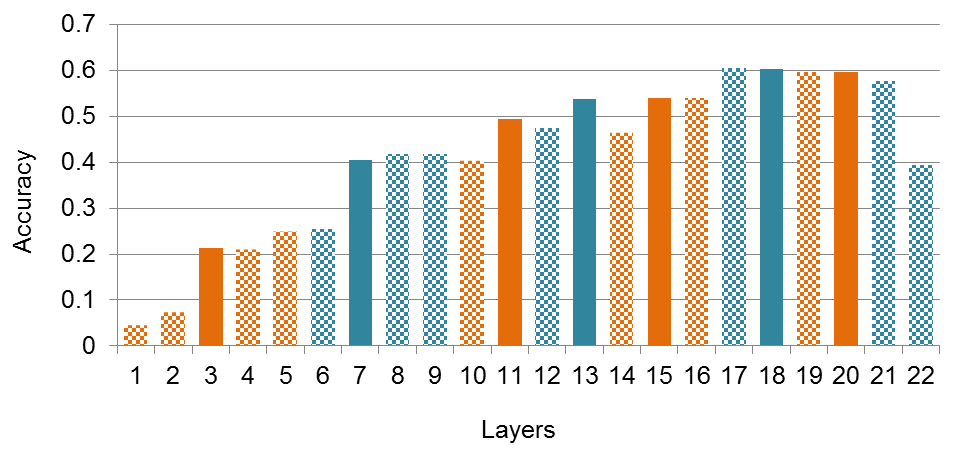
\includegraphics[width=\columnwidth]{fig/fig_layer_caffe.png}\label{fig:layer_deep19}}
\caption{The classification accuracy on MIT67~\cite{MIT67} using activations from each layer. We use a solid color fill representing the output of a ReLU layer. There are 7 ReLU layer for the Caffe model and 18 for Deep19. We see tend to see a performance jump at each successive RelU layer, particularly earlier on in the model.}
\label{fig:layer_MIT67}
\end{figure}


%Concretely, to compute the proposed representation, let $\alpha_i$ of dimension $w\times h\times k$ be the output of ReLU at $i$-th layer ($w=h$ in most CNN models). Each $w\times h$ is the Conv. response map of one of the $k$ filters. It carries the spatial activation information at the current scale. Thus, the \textit{orderless} response, $f_i$, at each scale can be computed by sum-pooling the first two dimension of $\alpha_i$, resulting in a $k$-dimensional vector, \ie,
%
%\begin{equation}
%f_i=\sum_w \sum_h \alpha_i
%\end{equation}


%-------------------------------------------------------------------------
%\subsection{Motivation: Classification Performance of Multi-scale CNN Activation\label{sec:multi}}

{\bf Multi-scale classification:} We now explore the use of multi-scale features. One immediate hurdle to including all features from all layers is the massive increase in dimensionality. We pursue two solutions. Firstly, we compute only marginal activations at each RelU layer with average pooling. We found average pooling to outperform sum pooling as the resulting marginal features remained in a reasonable dynamic range. For example, assume a particular layer was of size $H \times W \times F$, where $H$ is the height, $W$ is the width, and $F$ is the number of filter channels. We compute a $1 \times 1 \times F$ feature by averaing across spatial dimensions. Secondly, it may not be beneficial to add all layers, as they may encode redundant/correlated information (which may complicate learning by leading to overfitting). We search for an ``optimal'' combination of multiscale features with a greedy forward-selection strategy. We begin by initializing the set of included layers to the last RelU layer (a strong single-layer feature, as suggested by Fig.~\ref{fig:layer_MIT67}).
Fig.~\ref{fig:add_back} shows that performance increases as we add intermediate layers, while lower layers prove less helpful. 
% the performance increase in the beginning by adding mid-level features to enrich the model discriminativeness. However, including some low level responses to the feature actually hurts the performance, \ie, layer 7 and 3 in Fig.~\ref{fig:add_back_caffe}. 
Our observations suggest that high and mid-level features (\ie, \textit{parts} and \textit{objects}) are more useful than low-features based on \textit{edges} or \textit{textures}. 

%Since different CNN layers correspond to image feature at various scales, seen in Fig.~\ref{fig:moti}, we wonder whether combining activations at multiple scales help to extract a better feature. To address this question, we carried out another experiments on the MIT67 data~\cite{MIT67}. We start from the average-pooled response of the last ReLU layer and greedily concatenate the ones from previous ReLU layers. The reason we start from the last ReLU layer is that, in the literature when CNN is used for feature extraction, the response of the first fully connected layer is usually selected~\cite{cnn_baseline,Gong14}. Besides, our previous analysis in Fig.~\ref{fig:layer_MIT67} also demonstrates better discriminative power of high-level CNN layer.

%The rest of the experimental setups are the same as in Sec.~\ref{sec:indi_scale}, \ie, a set of 67-way one-vs-all linear SVM classifiers are trained every time we add one more layer. Since we keep on concatenating features at lower level, the feature dimension is monotonically increasing. As the results shown in Fig.~\ref{fig:add_back}, the performance increase in the beginning by adding mid-level features to enrich the model discriminativeness. However, including some low level responses to the feature actually hurts the performance, \ie, layer 7 and 3 in Fig.~\ref{fig:add_back_caffe}. We believe it demonstrates the benefit of incorporating more discriminative mid-level and high-level features of CNN (\ie, \textit{parts} and \textit{objects}), but not necessarily the low-level features, such as \textit{edge} or \textit{textures}. 

\begin{figure}[htbp]
\centering
	\subfigure[Caffe]{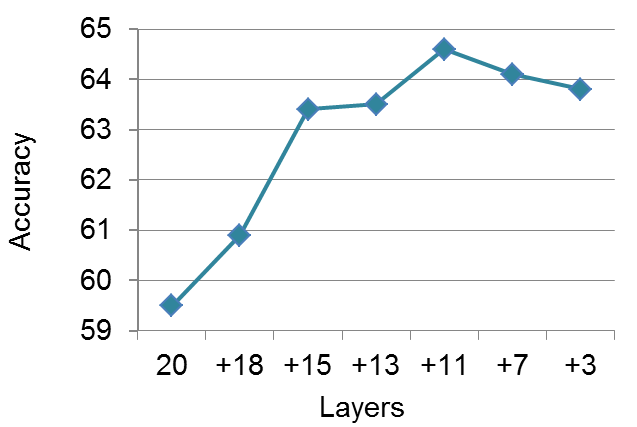
\includegraphics[width=.43\columnwidth]{fig/fig_add_back_caffe.png}\label{fig:add_back_caffe}}
	\subfigure[Deep19]{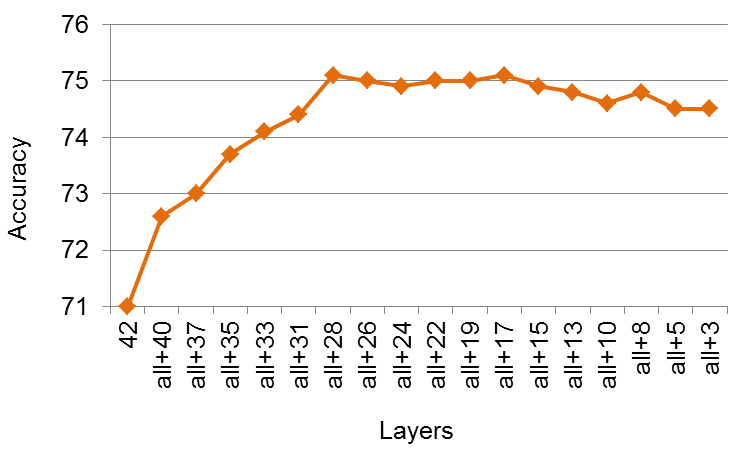
\includegraphics[width=.56\columnwidth]{fig/fig_add_back_deep19.png}\label{fig:add_back_deep19}}
\caption{The performance trend when incorporating more lower-level features. The keyword ``all'' means the previously added average-pooled ReLUs. \deva{Remove all. Why does Deep19 start with layer 42, while Fig3 suggests Deep19 has 20 layers?}. Performance increases as we add mid-layer features, while low-level features prove less helpful.}%performance drop is observed when incorporating more low level features.}
\label{fig:add_back}
\end{figure}

A more systematic way for select the correct scale to incorporate as feature is feature forward selection, \ie, greedily add the layer in the ReLU pool which results in the best performance boost in an iterative manner. As seen in Fig.~\ref{fig:forward_select_caffe}, the optimal results of this greedy approach is congruent with the previous results in Fig.~\ref{fig:add_back_caffe}, which rejects the low-level features. Similarly for the Deep19 model in Fig.~\ref{fig:forward_select_deep19}, although the feature pool is large (18 ReLU layers), the optimal greedy results includes only the mid- or high-level features. \deva{I don't understand the difference between Fig4 + 5?}

\begin{figure}[htbp]
\centering
	\subfigure[Caffe]{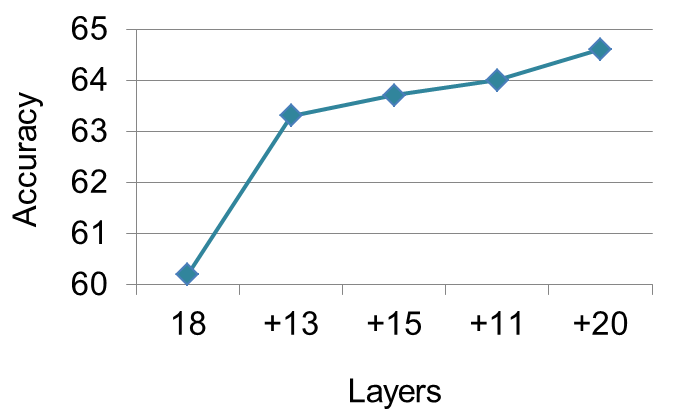
\includegraphics[width=.49\columnwidth]{fig/fig_forward_select_caffe.png}\label{fig:forward_select_caffe}}
	\subfigure[Deep19]{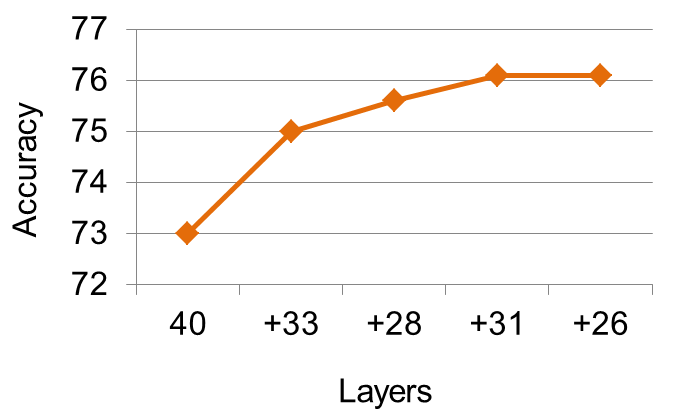
\includegraphics[width=.49\columnwidth]{fig/fig_forward_select_deep19.png}\label{fig:forward_select_deep19}}
\caption{The performance trend when using forward selection to incorporate $f$s from the ReLU layer. }

\label{fig:forward_select}
\end{figure}

{\bf Scale-specific retrieval:}  \deva{TODO. Refer to figure 2.}

For our latter analysis and experiments on other datasets, we use scales selected by the forward selection algorithm on MIT67 data. We use cross-validation data to select these scales, and use the same fixed set across all our benchmark datasets.

\subsection{Model\label{sec:model}}

Based on the analysis in Sec.~\ref{sec:indi_scale} and Sec.~\ref{sec:multi}, we propose a novel deep CNN architecture, Bag-of-Multi-Scale-Activation (BoMSA), shown in Fig.~\ref{fig:model}. A typical CNN layer consists of four layers, \ie, Conv., ReLU, contrast normalization (Norm), Max-pool layers (with the Norm and Max-pool layers being optional). This augmentation schema converts the traditional CNN \textit{chain} model~\cite{AlexNet,veryDeep} to a complex model by linking each ReLU to an average-pooled layer and FC layer thereafter. Before feeding into the Soft-max layer, an \textit{Add} layer is introduced to combine the responses from all FC layers. 

\begin{figure*}[t!]
\centering
	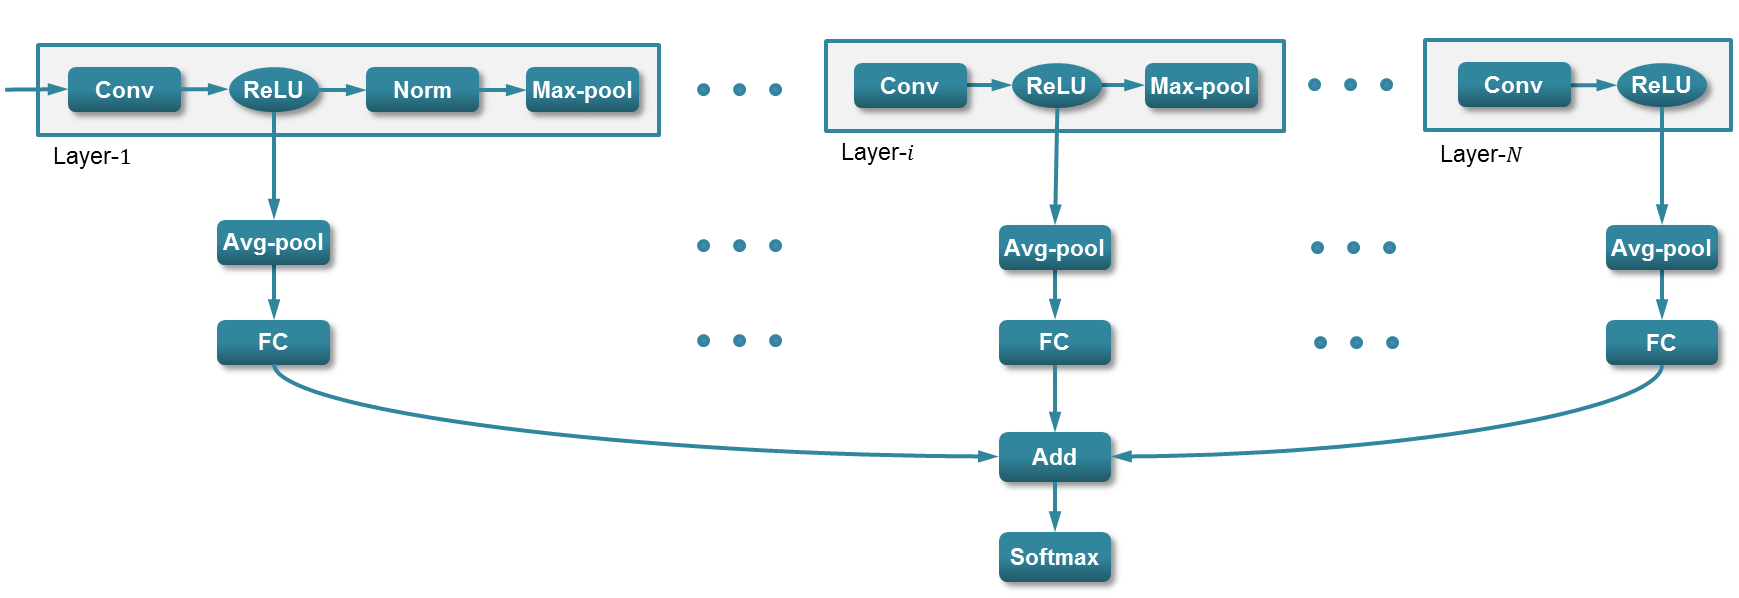
\includegraphics[width=\textwidth]{fig/fig_model.png}
\caption{Our multi-scale DAG-CNN architecture is constructed by adding (marginalized) multi-scale output connections to an underlying {\em chain backbone} from the original CNN.\deva{Change formatting to reduce verticle space (too much whitespace)}}
\label{fig:model}
\end{figure*}

\subsection{Training}

Let $\textbf{w}_1,...\textbf{w}_K$ be the CNN model parameters at $1,..,K$-th layer, training data be ($\textbf{x}^{(i)},\textbf{y}^{(i)}$), where $\textbf{x}^{(i)}$ is the $i$-th input image and $\textbf{y}^{(i)}$ is the indicator vector of the class of $\textbf{x}^{(i)}$. Then we intend to solve the following optimization problem

\begin{align}
\argmin_{\textbf{w}_1,...\textbf{w}_K} \frac{1}{n}\sum_{i=1}^{n} \mathcal{L}(f(\textbf{x}^{(i)};\textbf{w}_1,...,\textbf{w}_K),\textbf{y}^{(i)})
\end{align}

We adopt the stochastic gradient descent to minimize the objective function. For a traditional \textit{chain} model, the derivative of the objective function computed by chain rule results in the well-known back-propagation algorithm. In our proposed complex model, care need to be taken in the feed-forward for Add layer and back-propagation for all the ReLU layers. In the feed-forward step, the Add unit simply adds multiple inputs from all ReLU layers. In the back-prop step for $i$-th ReLU layer (seen in Fig.~\ref{fig:backprop_eq}), let $\alpha_i$ be its input, $\beta_i^{(j)}$ be the output for its $j$-th branching; $z$ is the final output of the Softmax layer. Thus, the gradient of $z$ with respect to $i$-th ReLU layer can be computed as

\begin{align}
\frac{\partial z}{\partial \alpha_i}=\sum_{j=1}^{C}\frac{\partial z}{\partial \beta_i^{(j)}}\frac{\partial \beta_i^{(j)}}{\partial \alpha_i}
\end{align}

\noindent where $C=2$ for our model. Each partial derivative component, $\frac{\partial z}{\partial \beta_i^{(j)}}\frac{\partial \beta_i^{(j)}}{\partial \alpha_i}$, can be computed in the typical back-prop fashion. 


\begin{figure}[htbp]
\centering
	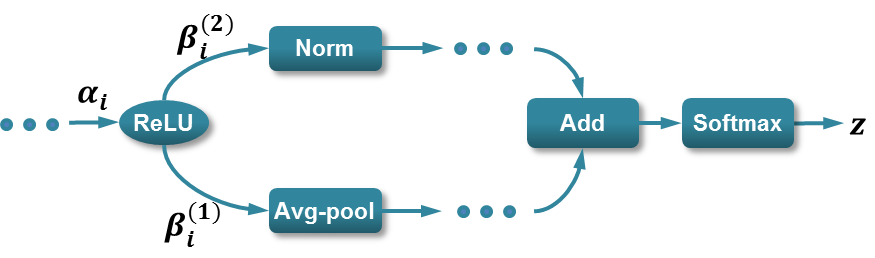
\includegraphics[width=\columnwidth]{fig/fig_backprop_eq.png}
\caption{Visualization of the parameter setup at $i$-th ReLU.}

\label{fig:backprop_eq}
\end{figure}


\section{Discussions\label{sec:ana}}

\subsection{off-the-shelf Model Instantiation}

We first point out an interesting instantiation of our model, linking back to the analysis in~\ref{sec:multi}. We could switch the softmax loss to hinge loss and freeze the back-prop at the FC layer. In this way, we prevent altering the chain-part of our model and only allow training on the augmented part our model, \ie, we learn an linear combination of the FC layers represents multi-scale ReLU activations. Thus, this is equivalent of training a SVM classifier based on the concatenation of the average-pooled activations at all ReLUs. As a result, we could extract multi-scale features using pre-trained CNN models such as the ones in~\cite{AlexNet, veryDeep} and use off-the-shelf SVM solver such as~\cite{liblinear} to train the augmented part our model.

\subsection{Relationship to the literature}

Our work is inspired by~\cite{Gong14}. In~\cite{Gong14}, local patches at three scales are first extracted (roughly 50 patches per image in their setting); each patch is then feed to an off-the-shelf CNN and the activations of the first fully connected layer (4096-dimension) are used for post processing, \ie, K-means + VLAD pooling. 

Our approach has several advantages over~\cite{Gong14}:
\begin{enumerate}
\item \cite{Gong14} computes multiple feed-forward on patches generated from a single image. Computing convolution is the bottleneck for this procedure. In our approach, our model is trained to adapt to multi-scale features. Thus, during test phase,
only one feed-forward computation is needed for one image. As matter of fact, extracting feature of one image in~\cite{Gong14} takes more than 20 seconds while ours only take less than 1 second for the augmented Caffe model. 

\item \cite{Gong14} uses K-means clustering algorithm in the VLAD pooling, which can generate inconsistent results due to random initialization. 

\item \cite{Gong14} conducts two steps of PCA (first PCA to reduce $4096$-dimensional activation to $500$-dimension, and second PCA to reduce $50,000$-dimensional VLAD pooled feature to $4096$-dimension). This can also be one bottleneck of their approach. 

\end{enumerate} 

%Overall, the implementation of \textit{multi-scale orderless} feature in~\cite{Gong14} is not only inefficient but also prone to over-fitting due to a number of hyper-parameter tuning. On the contrary, our implementation is easy to compute and little parameter tuning is needed. 

%-------------------------------------------------------------------------
\subsection{The Analysis of Invariance}

Besides the insight on visualizing deep CNN features,~\cite{visual_cnn} provides transformation invariance analysis of their model on several images. This is done by comparing the feature vector distance between the original and transformed images. Realizing that several examples do not necessarily represents the overall statistics,~\cite{Gong14} improve the invariance analysis by experiments on the SUN397 scene database~\cite{SUN397}. Unfortunately, only the results on 4 categories are provided in their paper. The performance for the entire dataset is still unknown.

To close the aforementioned gap and analyze the invariance of our representation, we carried out experiments on the entire MIT Indoor dataset~\cite{MIT67} and report the average performance. We intend to compare the tolerance to transformation of the our multi-scale feature compared with a single-scale CNN feature. Concretely, the single-scale CNN feature in comparison is the activation of a CNN model which achieves best classification performance (not necessarily the output of the first FC layer). For a fair comparison, the multi-scale features are extracted by concatenating the output of all sum-pooling layers. We first trained $67$-way one-vs-all linear SVM classifiers for all $67$ classes using features extracted from the original images. During test phase, four transformations are considered for the analysis, \ie, translation, scaling, flipping, and rotation. Fig.~\ref{fig:invar_eg} illustrates all the transformations and their corresponding parameters, which are similar to the ones in~\cite{Gong14}. 

After applying the transformations to test images, both multi- and single-scale features are extracted. The classification is conducted using the trained SVMs, and the accuracy is shown in Fig.~\ref{fig:invar_rst}. Each data point represents the performance on the entire test data. As seen in Fig.~\ref{fig:invar_rst}, the transformations almost always hurt the performance except for horizontal flip. This observation is similar to the one in~\cite{Gong14}. We also see that multi-scale feature consistently out-performs the single-scale feature under every degree of all transformations. As far as the invariance is concerned, we observe the similar level of performance decrease. This means that both features have the similar level of tolerance to transformations. This immediately suggest that ``training jittering'', \ie, including transformations in the training data, will improve the performance. 


\begin{figure}[htbp]
\centering
	\subfigure[v-translation]{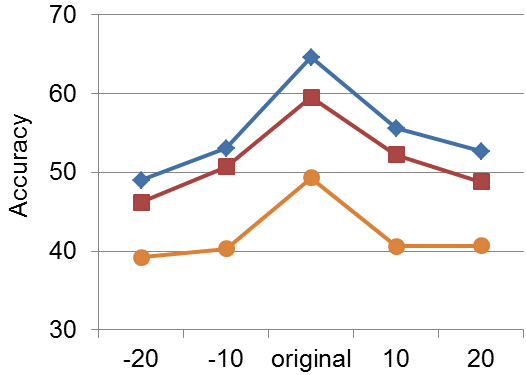
\includegraphics[width=.49\columnwidth]{fig/invar/v.png}\label{fig:inv_v}}
	\subfigure[scaling]{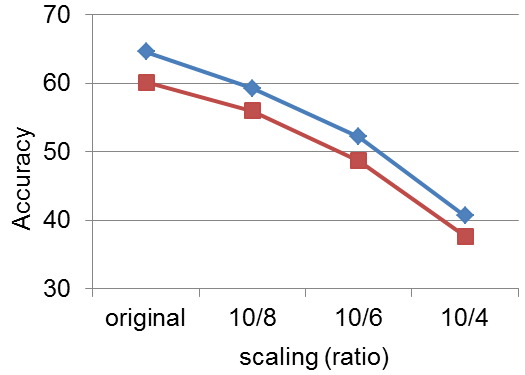
\includegraphics[width=.49\columnwidth]{fig/invar/s.png}\label{fig:inv_s}}
	\subfigure[h-translation]{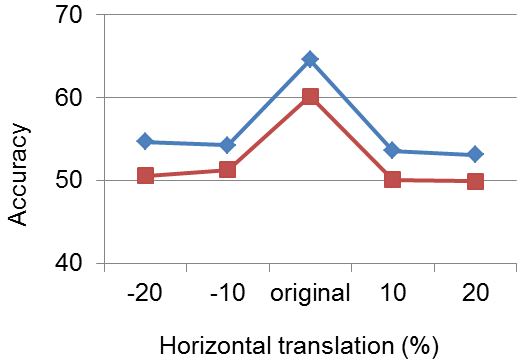
\includegraphics[width=.49\columnwidth]{fig/invar/h.png}\label{fig:inv_h}}
	\subfigure[flipping]{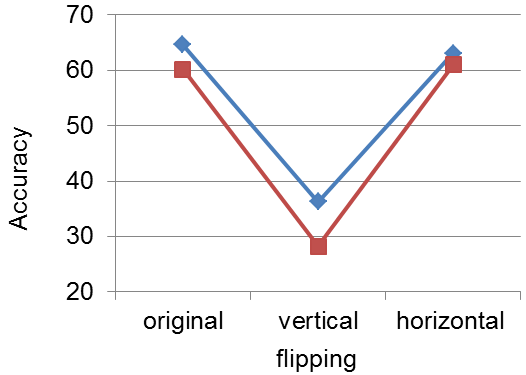
\includegraphics[width=.49\columnwidth]{fig/invar/f.png}\label{fig:inv_f}}
	\subfigure[rotation]{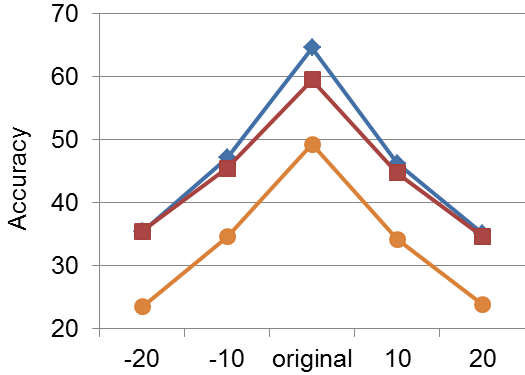
\includegraphics[width=.49\columnwidth]{fig/invar/r.png}\label{fig:inv_r}}

\caption{The classification accuracy of various transformations on test images in MIT67 data~\cite{MIT67}. The legends shown in Fig.~\ref{fig:inv_v} is the same in the other four figures.}

\label{fig:invar_rst}
\end{figure}

%-------------------------------------------------------------------------
%-------------------------------------------------------------------------
\section{Experimental Results\label{sec:exp}}

In this section, we conduct experiments on benchmark datasets, SUN397~\cite{SUN397}, MIT67~\cite{MIT67}, and Scene15~\cite{Scene15}, and show consistent performance increase using our approach. 

\subsection{Experiment Setup}

We should first stress that our augmentation is applied to the ReLU layers selected based on MIT67 dataset, as shown in Fig.~\ref{fig:forward_select}. The learned structure for both Caffe and Deep19 is then applied to all the experiments in this Section, demonstrating the data-independence of our approach. 

We follow the standard image pre-processing steps in the literature~\cite{AlexNet,Caffe,veryDeep}. Since both Caffe~\cite{Caffe} and Deep19 models~\cite{veryDeep} have a fixed input size of $224\times 224$, we first resize the image such that the smaller side matches $224$, and then crop an $224\times 224$ patch from the center. The mean RGB value of each model learned on ImageNet~\cite{ImageNet} is then subtracted.  

We show results of using our BoMSA augmented model for feature extraction. Thus, the output of all the average-pooled ReLU activations are concatenated as our multi-scale representation. For a fair comparison, we compare the multi-scale feature to the best performing single-scale feature. All features are $l2$-normalized. Then the off-the-shelf linear SVM solver~\cite{liblinear} is used to train 67-way one-vs-all classifiers with no parameter tuning.


%-------------------------------------------------------------------------
\subsection{SUN397}

SUN397~\cite{SUN397} is a large scene recognition dataset with 397 categories, each of which includes more than 100 images. The total number of images exceeds 100k. The average classification accuracy is usually report from a 10-fold cross validation. The split file is provided in~\cite{SUN397} with 50 images for training and the rest being test for each fold.  


\begin{table}
\begin{center}
\begin{tabular}{|l|c|}
\hline
Approach & Accuracy(\%) \\
\hline
Deep19-BoMSA & \textbf{55.5} \\
Deep19-single & 51.9 \\
Caffe-BoMSA & 46.6	\\
Caffe-single & 43.5 \\ \hline
MOP-CNN~\cite{Gong14} & 52.0 \\
Places~\cite{Places}	& 54.3	\\
DeCaf~\cite{DeCaf} & 40.9	\\
FV~\cite{FV} & 47.2 \\
Baseline~\cite{SUN397} & 38.0 \\
\hline
\end{tabular}
\end{center}
\caption{Classification results on SUN397}
\label{table:SUN397}
\end{table}

<Improvement over pre-trained models>
<Achieves best performance>
<talk about Places, using different data -> model structure and better domain specific data are both important>


%-------------------------------------------------------------------------
\subsection{MIT67}

MIT67 refers to the MIT Indoor~\cite{MIT67} scene classification for 67 categories. Indoor scenes depends on highly variable features to describe them. There are cases that can be well characterized by high-level spatial geometry (\eg church and cloister) and low-level textures (\eg wine celler and library). Our multi-scale model is designed to encode feature at all levels, and thus, enable us to learn both high- and low-level statistics of scene categories. The training/test split is made available and there are 80/20 training/test images for each class.

\begin{table}
\begin{center}
\begin{tabular}{|l|c|}
\hline
Approach & Accuracy(\%) \\
\hline
Deep19-BoMSA & \textbf{76.1} \\
Deep19-single & 70.8 \\
Caffe-BoMSA & 64.6	\\
Caffe-single & 59.5 \\ \hline
MOP-CNN~\cite{Gong14} & 68.9 \\
Places~\cite{Places}	& 68.2	\\
Mid-level~\cite{mid_level} & 64.0	\\
FV+BoP~\cite{FV_BoP} & 63.2 \\
Disc. Patch~\cite{disc_patch} & 49.4 \\
SPM~\cite{spatial_pyramid} & 34.4	\\
\hline
\end{tabular}
\end{center}
\caption{Classification results on MIT67}
\label{table:MIT67}
\end{table}


%-------------------------------------------------------------------------
\subsection{Scene15}



%-------------------------------------------------------------------------
%-------------------------------------------------------------------------
\section{Conclusion}




{\small
\bibliographystyle{ieee}
\bibliography{mobib}
}

\end{document}
